\documentclass[]{report}

\usepackage[utf8]{inputenc}
\usepackage[spanish]{babel}
\usepackage{graphicx}
\graphicspath{{imagenes/}}
\usepackage[colorlinks]{hyperref}
\usepackage[svgnames]{xcolor}
\hypersetup{citecolor=DarkRed}
\hypersetup{linkcolor=DarkBlue}
\hypersetup{urlcolor=DarkBlue}

% Title Page
\title{Agrupamiento difuso}
\author{Carlos Cobos Suárez\\Adrián Morente Gabaldón}


\begin{document}
\maketitle

\begin{abstract}
	
	Este trabajo versa sobre el ámbito de la ciencia de datos y consiste en exponer las limitaciones del agrupamiento o \textit{clustering} clásico para resolverlas tras estudiar cómo la lógica difusa puede ayudar en la modelización del problema.\\
	
	Se darán a conocer los distintos tipos de modelos de agrupamiento usando lógica difusa, así como sus características y limitaciones intentando resolverlas con otro tipo de modelos.\\
	
	Para terminar y entender que los modelos expuestos tienen una gran relevancia en nuestra sociedad, así cómo destacar cómo el agrupamiento difuso (o \textit{fuzzy clustering}) está presente en nuestros días, se citarán aplicaciones reales que hacen uso de estos modelos.\\
	
\end{abstract}

	\chapter{Agrupamiento clásico}
	
		\section{Definición}
		
			Entendemos por \textbf{agrupamiento clásico} a la técnica de clasificación de datos en distintas categorías según su similitud (o \textit{distancia}, si los entendemos como una representación de puntos en un espacio determinado).
			
			\begin{figure}[h]
				\centering
				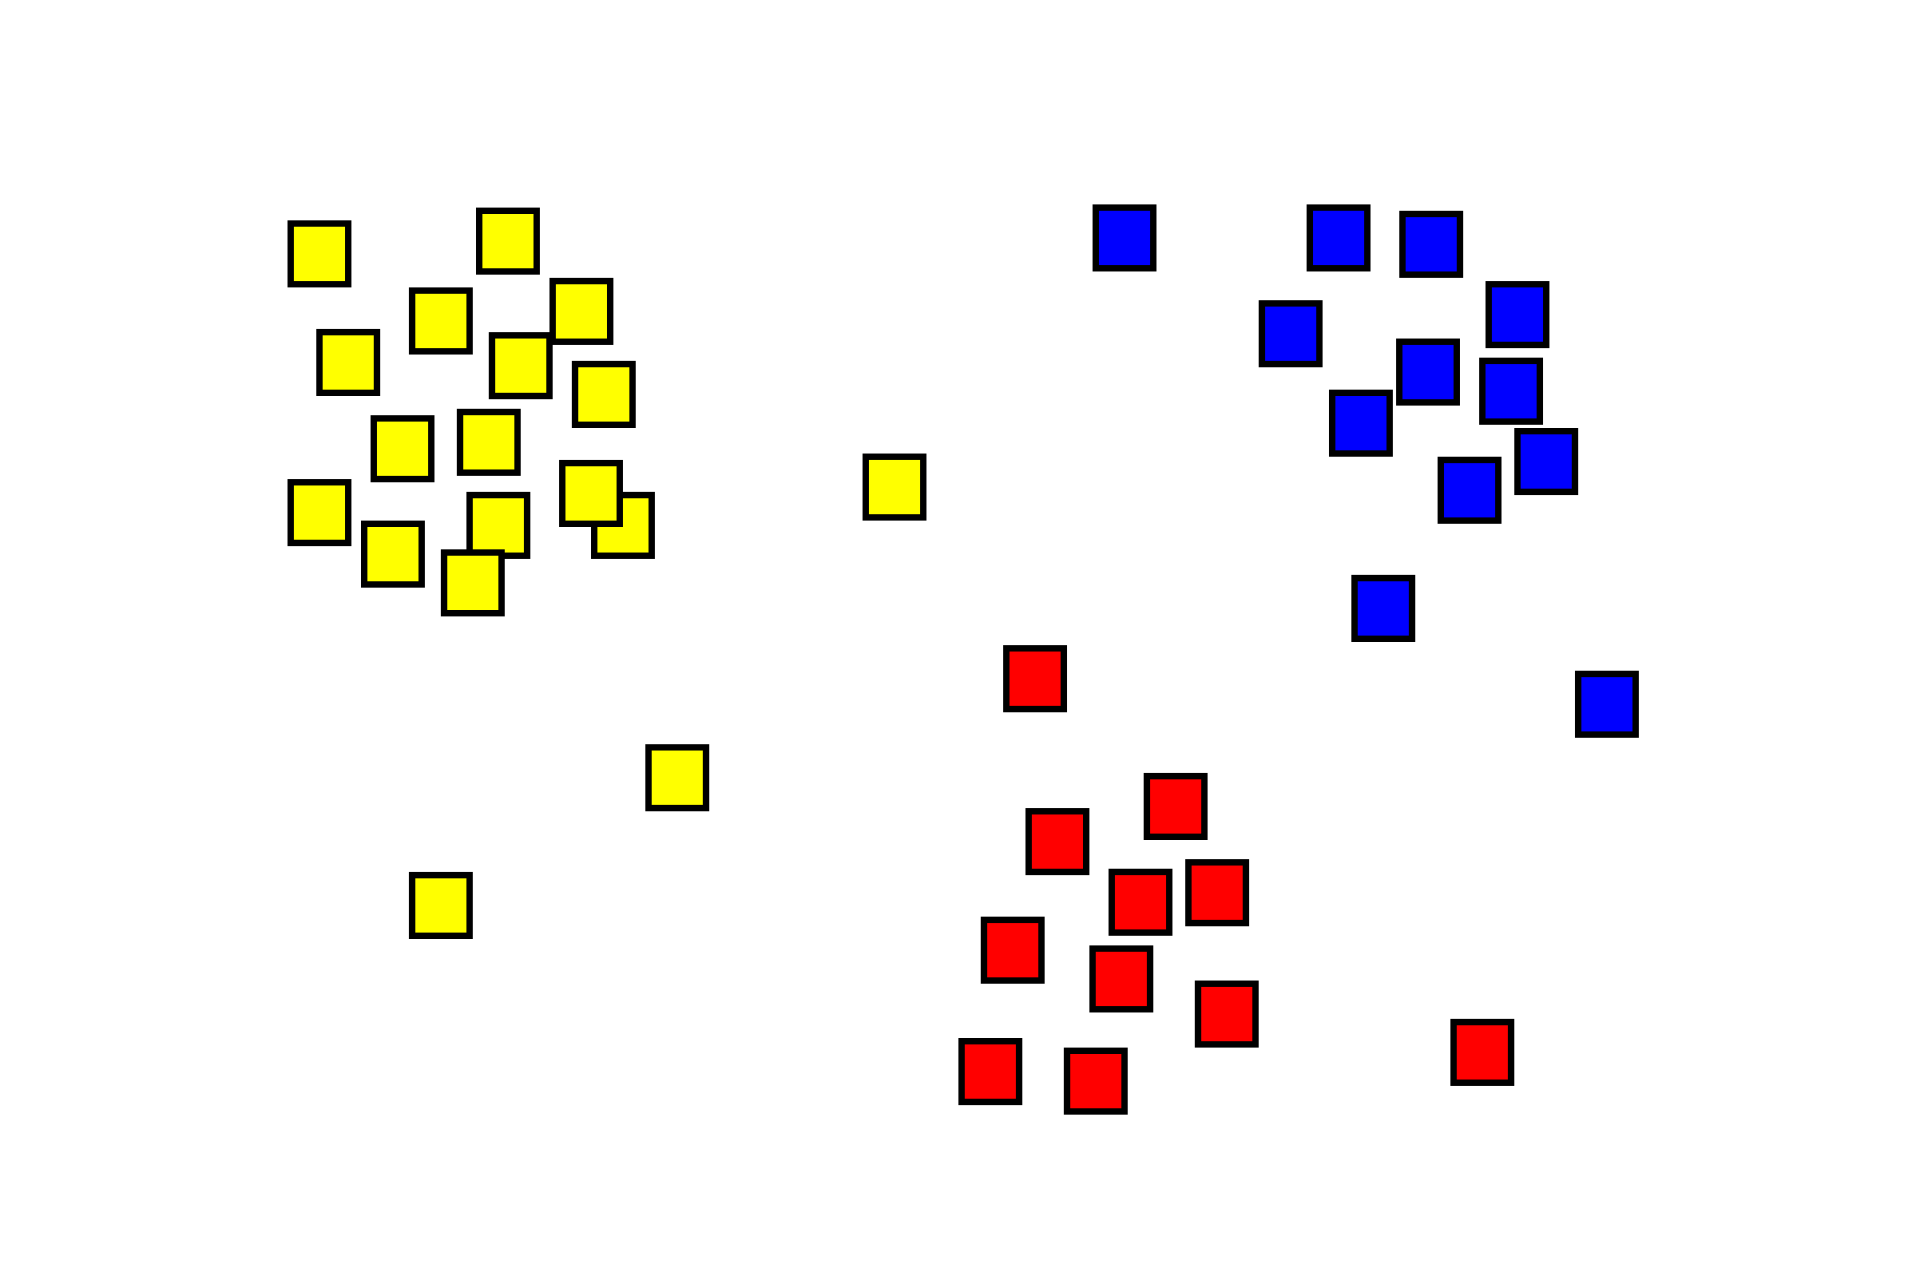
\includegraphics[width=0.5\textwidth]{clustering.png}
				\label{clustering1}
				\caption{Ilustración de agrupamiento clásico. \href{https://en.wikipedia.org/wiki/Cluster_analysis\#/media/File:Cluster-2.svg}{ \textit{(Wikimedia Creative Commons)}}}
			\end{figure}
		
			Se trata de una tarea principal en la labor de minería de datos a modo exploratorio, además de una técnica común para análisis estadístico de datos (aprendizaje automático, reconocimiento de patrones, análisis de imágenes, etc.).
					
		\section{Conceptos}
		
			Para entender con mayor profundidad los fundamentos del \textit{clustering}, deben interiorizarse algunos conceptos clave:
			
			\begin{itemize}
				\item \textbf{Clúster \textit{(o cluster)}}: se trata de cada una de las categorías o grupos en los que se clasifican finalmente los datos. Esto es, según vemos en la figura \ref{clustering1}, los distintos colores que identifican a cada grupo.
				\item \textbf{Centroide}: se conoce como tal al punto de referencia de cada \textit{cluster}, es decir, el elemento más representativo que comparte mayor similitud con el resto.
				\item \textbf{Función de distancia}: es la relación que indica el grado de disimilaridad entre los elementos del conjunto analizado; siendo mayor la similitud entre ellos cuanto menor sea esta \textit{distancia}, considerando a los individuos como vectores en el espacio de las variables. Puede calcularse mediante \textit{distancia euclídea}, \textit{distancia Hamming} o \textit{correlación de Pearson} entre otras.
				\item \textbf{Núcleo o \textit{kernel}}: son clases de algoritmos para análisis de patrones, donde la tarea general es encontrar y estudiar tipos de relaciones en conjuntos de datos. En su definición más simple, implican la transformación de datos en otras dimensiones cuyo margen divisorio de los elementos es más acentuado y permite una visualización y categorización más claras.
			\end{itemize}
		
		\section{Modelos de agrupamiento clásico}
		
			Durante el estudio de conjuntos de datos basado en agrupamientos y/o categorización, se pueden seguir diversos modelos que condicionarán el contenido de los grupos resultantes. Esto es, el resultado diferirá en función del criterio seguido para asignar una categoría u otra a cada uno de los datos presentes en el conjunto. Veamos algunos de los modelos posibles:
		
			\begin{itemize}
				\item \textbf{Conectividad}: el criterio seguido para categorizar cada uno de los elementos se corresponde con la cercanía que tenga un determinado dato con el resto. Por ejemplo, si en un espacio tridimensional un dato sin categoría se encontrase a una distancia euclídea de 10 de un elemento de clase A, y a una distancia 5 de un dato de clase B; se inferiría que el elemento estudiado comparte más similitud con los datos de la segunda clase, y se categorizaría dentro de ella.
				\item \textbf{Basado en centroide}: en este caso, se seguiría una especie de modelo guiado por conectividad con la salvedad de que las distancias se calcularían respecto a cada uno de los centroides presentes en el modelo, y dicho elemento se clasificaría dentro de la clase a la que está asignado el centroide más cercano.
				\item \textbf{Basado en distribuciones}: es el más estrechamente ligado a los modelos y fundamentos estadísticos. Los clústeres son definidos por objetos que pertenecen mayormente a la misma distribución. Producen modelos complejos con que capturar correlación y dependencia entre atributos de los datos estudiados. A menos que se establezcan unos límites sobre la complejidad del modelo, el \textit{sampling} de datos aleatorios de forma estadística puede afectar negativamente causando \textbf{sobreajuste}.
				\item \textbf{Basado en densidad}: en este modelo, los grupos son definidos a modo de áreas donde la densidad de datos es mayor que en el resto del conjunto. Los objetos que se encuentran esparcidos por el espacio sin acercarse a ningún área, se consideran \textit{ruido} o \textbf{puntos frontera}.
			\end{itemize}
		
		\section{Proceso y algoritmo}
		
			El proceso de clasificación de datos en clases es relativamente sencillo, y se puede explicar de forma ejemplificada según el conocido algoritmo \textbf{\textit{K-means}} (o \textit{K-medias} en español), que asigna clases a los datos no categorizados en función del centroide más cercano:
		
			\begin{figure}[h]
				\centering
				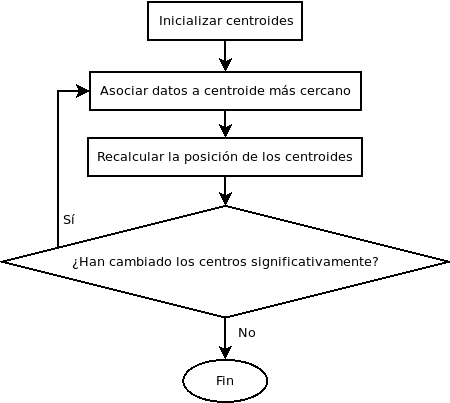
\includegraphics[width=0.7\textwidth]{agrupamiento-clasico.png}
				\label{clustering-algorithm}
				\caption{Proceso de agrupamiento clásico}
			\end{figure}
		
			Describamos ligeramente el proceso ilustrado arriba:
			
			\subsection{Inicialización de centroides}
			
				Consiste en colocar los centroides de forma generalmente aleatoria, dado que tomarán una posición más relevante a lo largo del proceso, conforme se vayan asignando datos a sus clases.\\
				
				La decisión más importante aquí es el número de centroides que se utilizan, aunque esta decisión goza de fácil solución si repetimos el algoritmo para distinto valor de este número, como podemos ver en la siguiente imagen:
				
				\begin{figure}[h]
					\centering
					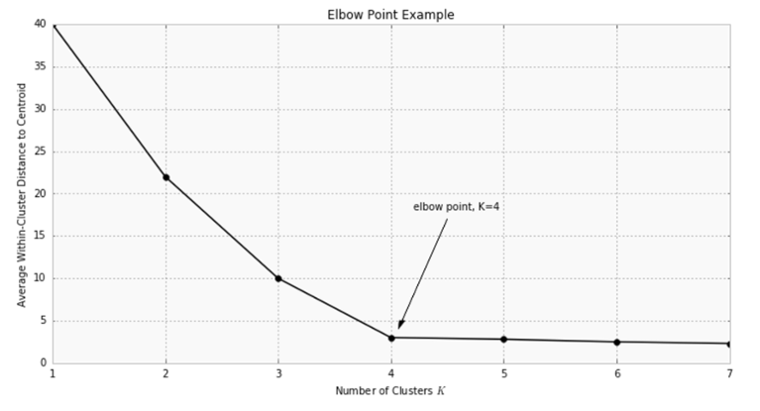
\includegraphics[width=0.9\textwidth]{k-means-oracle.png}
					\label{k-means-elbow-point}
					\caption{Inferencia del número idóneo de centroides a usar en un estudio de agrupamiento - \href{https://www.datascience.com/blog/k-means-clustering}{\textit{Oracle+DataScience}}}
				\end{figure}
				
				La opción más general reside en repetir el proceso del algoritmo aumentando ligeramente el número de centroides usados, hasta llegar al punto de inflexión donde aumentar este valor no produce una mejora demasiado notable, dado que conforme se incrementa el valor \textit{K}, así lo hace la capacidad computacional requerida para tratar el problema.
				
			\subsection{Clasificación de datos según centroide más cercano}
			
				Para seguir el modelo basado en centroide, cada uno de los datos presentes en el conjunto se asocia a la clase de la que es representativo el centroide más cercano o similar a dicho dato. Dependiendo del algoritmo, este criterio de asignación a categorías obviamente diferiría en cierto aspecto, pudiendo basarse esta decisión en alguna función de distancia de las comentadas previamente.
			
			\subsection{Reposicionamiento de los centroides}
			
			\subsection{Condición de parada}
				
		\section{Limitaciones}
		
			Lógicamente, estas aproximaciones basadas en agrupamiento clásico sufren de algunas limitaciones:
			
			\begin{itemize}
				\item Cada uno de los datos del conjunto solo pueden pertenecer a un \textit{cluster} (o lo que es lo mismo, ser asignados a una clase). Lógicamente no se contempla la posibilidad de que un elemento pueda compartir similitud gradual con diversas categorías, lo que aleja el estudio de los datos de la posible solución más favorable o descriptiva.
				
				\begin{figure}[h]
					\centering
					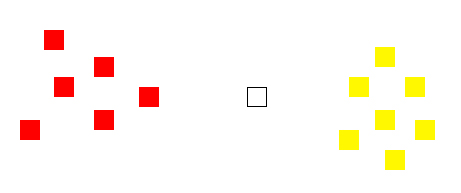
\includegraphics[width=0.5\textwidth]{Artboard1.jpg}
					\label{clustering2}
					\caption{Problema en la asignación de un dato en clustering clásico. ¿Qué categoría asignar al punto blanco?}
				\end{figure}
			
				\item Los mecanismos de exploración y clasificación de los datos no aseguran \textbf{convergencia}. El continuo cálculo de los centroides podría mantenerse eternamente efectuando las mismas operaciones repetitivas cuyo reposicionamiento de estos datos representativos alternase siempre de igual forma. Si existiese un mecanismo que permitiese relajar esta limitación, la inferencia extraída finalmente del estudio sería más descriptiva y ajustada a los datos reales.
			\end{itemize}
	
	\chapter{Agrupamiento difuso}
		Tal y como se acaba de ver, el agrupamiento clásico tiene una limitación bastante importante y es la de que un sólo dato puede pertenecer a un \textit{cluster}. Esto también tiene la consecuencia de que, dependiendo del algoritmo de agrupamiento que se vaya a emplear, no se puede garantizar la convergencia del mismo.
		
		A demás, si se usan redes neuronales para llevar a cabo la labor de agrupar los datos, es natural y lógico pensar que un sólo dato va a provocar la activación de más de una neurona. Es por ello que se tiene que cambiar el modelo clásico a uno más permisivo en el cual se solucionen dichos problemas.
			
		\section{Definición}
			Como se ha dejado entrever, el agrupamiento difuso permite que un dato pueda pertenecer a varios \textit{clusters} a la vez. Esto es posible debido a que al modelo clásico se le añade el concepto de \textit{función de pertenencia} que es propio de la lógica difusa.
			
			De hecho, en este modelo, un dato tiene $C$ grados de pertenencia, siendo $C$ el número de \textit{clusters} en los que se quiere agrupar los datos. La única limitación que tiene este modelo es que la sumatoria de los grados de pertenencia de un dato tiene que ser 1, es decir:
			
			$$\sum_{i=1}^c\mu_i(x_j) = 1, \forall j$$
			
			luego: $0 \leq \mu_i(x) \leq 1, \forall i=1,...,C$, es decir, el grado de pertenencia de cualquier dato en un \textit{cluster} tiene que estar en el intervalo cerrado [0,1].
			
			No obstante, la función que el agrupamiento clásico quiere minimizar no varía en su esencia:
			
			$$J_m(U,v) = \sum_{k=1}^n \sum_{i=1}^c (u_{ik}^m d^2_{ik}$$

			siendo:
			\begin{itemize}
				\item $d^2_{ik}$ la distancia entre los elementos y los centroides de los grupos.
				\item $(u_{ik})^m$ el grado de pertenencia asociado a cada distancia elevado a la m-ésima potencia. Cuando $m$ tiende a 1 ($m \rightarrow 1$) el modelo funcionaría cada ves más como un modelo clásico, mientras que si $m \rightarrow \infty$ el modelo no daría ningún resultado debido a que el grado de pertenencia de todos los elementos sería $1/C$.
			\end{itemize}
						
			El ejemplo anterior que no se ha podido resolver con el modelo clásico, se va a tratar de resolver con este nuevo enfoque. Como se vio en el ejemplo, el dato situado en medio de los dos grupos no se sabía a cual de ellos pertenecía. 
			
			Ahora, tras meter grados de pertenencia se puede resolver de manera trivial como se muestra en la siguiente figura:
			
			\begin{figure}[h]
				\centering
				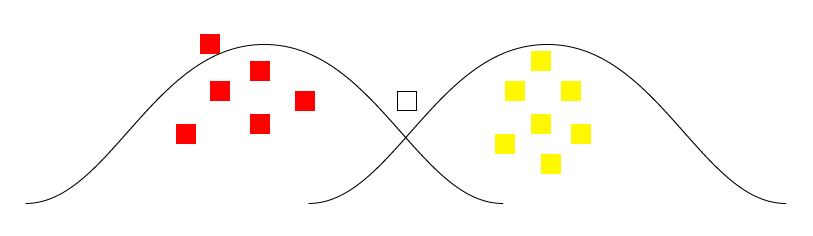
\includegraphics[width=0.5\textwidth]{clustering_difuso.jpg}
				\label{clustering_difuso}
				\caption{Ilustración de ejemplo de Agrupamiento Difuso. \href{https://github.com/adrianmorente/ExposicionClusteringDifuso/blob/master/doc/imagenes/clustering\_difuso.jpg}{ \textit{(Ilustración propia)}}}
			\end{figure}
		
			Como se puede observar gráficamente en la figura \ref{clustering_difuso}, cada \textit{cluster} forma una función de pertenencia centrada en el \textit{centroide} del mismo. Conforme se aleja del \textit{centroide} la función de pertenencia disminuye y se puede observar como el dato que se encuentra entre los dos grupos toma el mismo valor de pertenencia en los dos grupos.
			
			Este hecho nos da información de que realmente ese dato se clasificaría diferente si se aumenta el números de \textit{clusters} a 3. Para entender esto se propone el siguiente ejemplo. 
			
			Imaginemos que se quieren agrupar vehículos en dos clases: una clase \textit{turismo} y otra \textit{camión}. En el momento de clasificar una \textit{furgoneta}, sería imposible clasificarla en uno de estos dos grupos debido a que, en realidad, una \textit{furgoneta} es una mezcla entre un \textit{turismo} y un \textit{camión}, lo que sería otra clase distinta a estas.
		\section{Limitaciones}
	
	\chapter{Agrupamiento difuso posibilístico}
	
		\section{Definición}
	
	\chapter{Aplicaciones reales}
	
\bibliographystyle{plain}
\bibliography{citas}

\end{document}          
